\documentclass[tikz]{standalone}
% \documentclass{article}
\usepackage[utf8]{inputenc}
\usepackage{tikz}

\definecolor{sasaki}{HTML}{EF9AAF}
\definecolor{gibara}{HTML}{FFBE5C}
\definecolor{warabeda}{HTML}{E34E4F}
\definecolor{roa}{HTML}{D8368D}
\definecolor{toko}{HTML}{9D3757}
\definecolor{debiru}{HTML}{444C7D}

\begin{document}
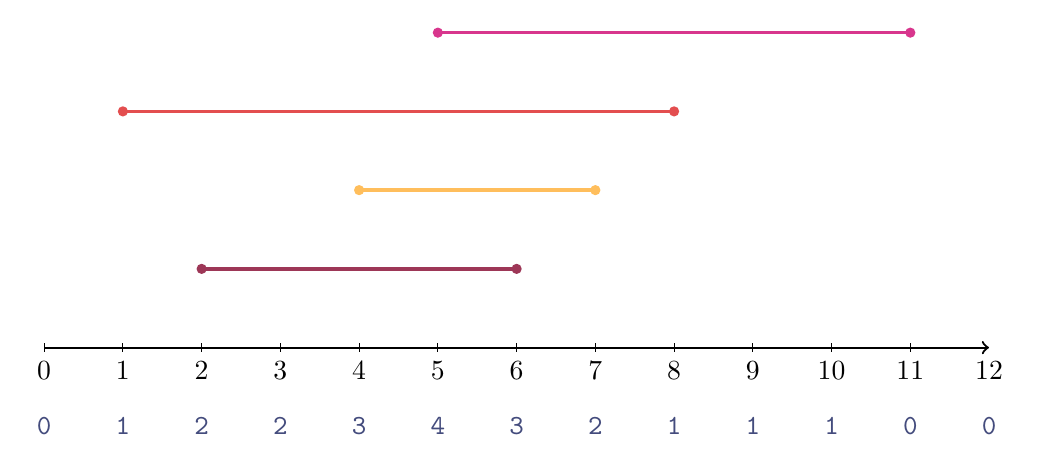
\begin{tikzpicture}
    % \draw[step=1cm,gray,ultra thin] (-0.9, -0.9) grid (12.9, 4.9);
    
    \draw[thick, ->] (0, 0) -- (12, 0);
    \foreach \x in {0, 1, ..., 11}
        \draw (\x cm, 1.5pt) -- (\x cm, -1.5pt) node[anchor=north] {$\x$};
    \draw (12, -1.5pt) node[anchor=north] {12};
        
    \draw[toko, very thick] (2, 1) -- (6, 1);
    \filldraw[toko, very thick] (2, 1) circle (1.2pt);
    \filldraw[toko, very thick] (6, 1) circle (1.2pt);
    
    \draw[gibara, very thick] (4, 2) -- (7, 2);
    \filldraw[gibara, very thick] (4, 2) circle (1.2pt);
    \filldraw[gibara, very thick] (7, 2) circle (1.2pt);
    
    \draw[warabeda, very thick] (1, 3) -- (8, 3);
    \filldraw[warabeda, very thick] (1, 3) circle (1.2pt);
    \filldraw[warabeda, very thick] (8, 3) circle (1.2pt);
    
    \draw[roa, very thick] (5, 4) -- (11, 4);
    \filldraw[roa, very thick] (5, 4) circle (1.2pt);
    \filldraw[roa, very thick] (11, 4) circle (1.2pt);
    
    \foreach[count=\x from 0] \y in {0, 1, 2, 2, 3, 4, 3, 2, 1, 1, 1, 0, 0}
        \draw (\x, -1) node[debiru] {\texttt{\y}};
    
\end{tikzpicture}
\end{document}
